\documentclass{article}
\title{Nechyba Ch.7 消费者商品市场的收入与替代效应}
\author{Dawei Wang}
\date{\today}
\usepackage{ctex}
\usepackage{amsmath}
\usepackage{amssymb}
\usepackage{graphicx} %插入图片的宏包
\usepackage{float} %设置图片浮动位置的宏包
\usepackage{subfigure} %插入多图时用子图显示的宏包
\begin{document}
	\maketitle
行为/选择,产生于当偏好面对环境随着个体在给定的处境下尽力做到“最好”时。

\section{收入和替代效应的图示阐述}
有两个主要的使选择集(从而使我们的经济环境)变化的方式:

第一,收入或财富的改变可以移动我们的预算约束而不改变它们的斜率,从而没有改变我们消费的不同商品的机会成本;

经济中个体——不管是以商品的价格、工资还是利率的形式——可能改变并且改变了预算约束的斜率与我们面对的机会成本。

\subsection{收入的变化对行为的影响}
禀赋变化(或外生收入变化)时,我们对商品的消费的变化完全取决于偏好的本质,以及表示我们偏好的无差异曲线图。

在分析选择集的大小由外生给定的收入决定的模型时,称收入变化的影响为收入效应(income effect);当选择集的大小由禀赋的价值决定时,称禀赋变化的影响为财富效应(wealth effect)。

整体上我们应该理解的是收入效应和财富效应都是指产生于一个预算约束的平行的移动对消费者决策的影响,这种移动并不包括机会成本的变化。

\subsubsection{正常品与低档品}

低档品/劣质品(inferior goods):收入效应为负——需求的收入弹性<0;

正常品(normal goods):收入效应为正——需求的收入弹性>0。

拟线性偏好:收入效应为0,介于正常品和低档品之间——需求的收入弹性=0。

\hspace*{\fill}

一旦观察到了对所有消费的一种商品存在负的收入效应,那么对消费的另一种商品一定存在正的收入效应。

\subsubsection{奢侈品与必需品}

奢侈品(luxury goods):收入需求弹性大于1;

必需品(necessity goods):收入需求弹性小于1。

位似偏好:收入需求弹性等于1,介于奢侈品和必需品之间。

\subsection{改变机会成本对行为的影响}

只要机会成本或价格变化,替代效应就会产生。

替代效应:

价格变化所引起的替代效应是纯粹地由机会成本的变化而不是由实际收入的变化所导致的行为的变化。

实际收入(real income)指实际福利(real welfare),因此“没有实际收入的变化”应该意指“没有效用的变化”或“没有无差异曲线的变化”。

\hspace*{\fill}

替代效应的方向总是朝着更多消费变得相对便宜的商品,并偏离变得相对昂贵的商品。

\hspace*{\fill}

尽管替代效应的方向是明确的,但该效应的大小完全依赖一个消费者潜在的偏好类型——该偏好的替代弹性大小。一个消费者的偏好的替代弹性越小,产生于机会成本变化的替代效应就越小。

\hspace*{\fill}

“Hicks”与“Slutsky”替代效应:

Hicks替代:没有无差异曲线的变化(效用不变);

Slutsky替代:购买初始消费束的能力不变。

\subsection{价格变化:结合收入和替代效应}

\begin{figure}[H] %H为当前位置,!htb为忽略美学标准,htbp为浮动图形
	\centering %图片居中
	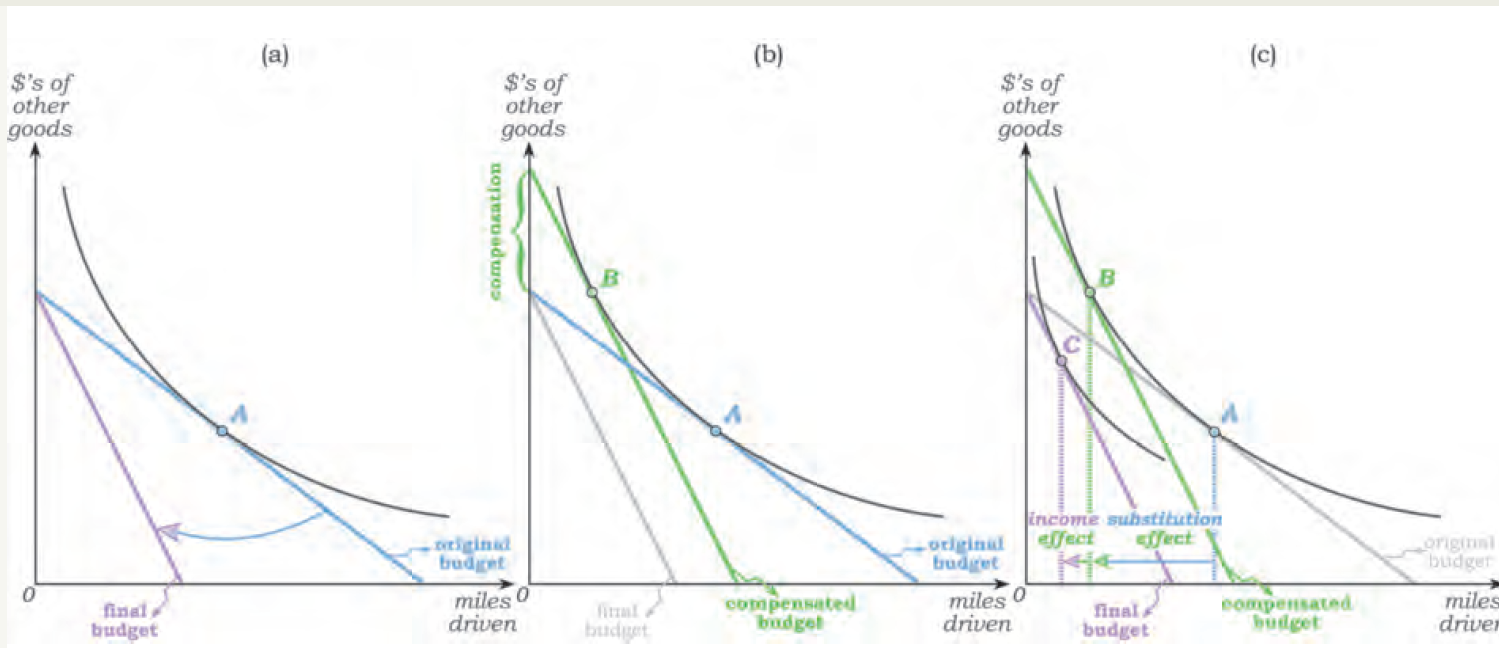
\includegraphics[width=1\textwidth]{substitution_7_5} %插入图片,[]中设置图片大小,{}中是图片文件名
	\caption{Substitution Effect} %最终文档中希望显示的图片标题
	\label{Fig.main2} %用于文内引用的标签
\end{figure}

价格变化的补偿约束是将新的价格考虑在内,但是包括充分的货币补偿以使消费者与价格变化前一样好的预算。若收入是外生的,补偿预算在价格上涨时要求正的价格补偿,反之反是。

\hspace*{\fill}

正常低档品与吉芬品:

低档品可以分为两类:随着价格上涨消费减少的低档品以及随着价格上涨而消费增加的低档品,称前者为正常低档品(regular inferior goods)而后者为吉芬品(Giffen goods)。

吉芬品的收入效应(低档程度)大于其替代效应。

为了观测到吉芬品,我们必须观察到那种商品价格的变化(外生收入不变),由于吉芬品是消费与价格同向变化的商品(当收入为外生且不变时)。

\section{收入和替代效应的数学分析}

没有偏好使得一种特别的商品总是低档品,商品仅对无差异曲线图的一些部分是低档的。

奢侈品与必需品:需求的收入弹性=1(位似偏好)为界,两商品中必需品与奢侈品是伴生的。



\end{document}